\documentclass{scrartcl}
\usepackage[utf8]{inputenc}
\usepackage[ngerman]{babel}
\usepackage{graphicx}
\usepackage{xurl}
\usepackage{hyperref}

\title{Untersuchung der harmonischen Reihe}
\subtitle{Berichts-Handout Arbeitsblatt 3}
\author{Chantal Gerth, Alina Apel\\635838, 614787\\Gruppe 22}
\date{}

\begin{document}

\maketitle
\tableofcontents
\thispagestyle{empty}

\newpage

\section{Einführung und Motivation}
Im heutigen Zeitalter werden Computer in fast allen Lebensbereichen genutzt. Daher ist es besonders wichtig, dass der Computer korrekt rechnet. Leider tut er das nicht immer. Ein anschauliches Beispiel dafür ist die harmonische Reihe. Deswegen geht es in diesem Experiment darum, die Konvergenz der harmonischen Reihe mit verschiedenen Algorithmen und Datentypen zu untersuchen und dies mit dem analytischen Ergebnis zu vergleichen.

\section{Theoretische Grundlagen}
Die harmonische Reihe ist eine unendliche Reihe der Form
\[
\sum_{n=1}^{\infty} \frac{1}{n},
\]
die aus den Kehrwerten natürlicher Zahlen besteht. Mathematisch gesehen divergiert die harmonische Reihe, was bedeutet, dass die Summe der Reihe gegen Unendlich strebt, wenn die Anzahl der Terme zunimmt. Beim Berechnen der Partialsummen der harmonischen Reihe durch einen Computer kann es allerdings zu Rundungsfehlern kommen, die durch die begrenzte Genauigkeit der Fließkommazahlen verursacht werden. Je nach Datentyp wird n so groß und damit der auf die vorherige Partialsumme aufzuaddierende Summand so klein, dass die Bitmuster der entsprechenden Datentypen nicht mehr ausreichen, um diese numerisch kleine Zahl darzustellen. Der entsprechende Summand wird deshalb auf 0 gerundet. Für höhere n wird dann nur noch 0 aufaddiert, sodass die Folge der Partialsummen zu konvergieren scheint. Die Genauigkeit der Ergebnisse hängt dabei vom verwendeten Datentyp und Algorithmus ab. Je weniger Nachkommastellen das Bitmuster eines Datentyps darstellen kann, desto früher tritt das Problem auf. Schlussendlich trat in allen von uns untersuchten Beispielen diese Konvergenz auf, obwohl die Reihe selbst divergiert.

\section{Experiment}
Unser Programm \texttt{main.py} ist ein Experimentierskript für den Nutzer. Es gibt die Möglichkeit, eine gewisse Anzahl an Partialsummen zu berechnen, grafisch darzustellen und zu speichern/abzurufen. Dabei kann der Nutzer Standardparameter wählen oder eigene Parameter eingeben. Für die Berechnung wird ein Anfangswert und ein Endwert, sowie eine Basis benötigt. Dann kann der Nutzer wählen, wie viele Partialsummen er berechnet haben will. Anschließend berechnet das Programm durch Vorwärtssummation und Rückwärtssummation mit den Datentypen \texttt{np.float16}, \texttt{np.float32} und \texttt{np.float64} die Partialsummen.

\newpage
\section{Grafiken}

\begin{figure}[h]
    \centering
    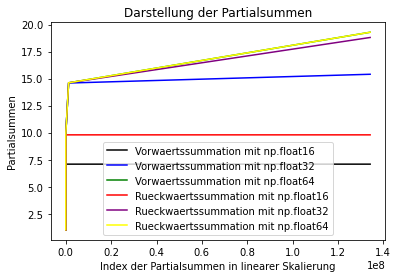
\includegraphics[width=0.6\textwidth]{plot_basis8_endwert9.png}
    \caption{Basis 8, Startwert 0, Endwert 9, Num 5}
\end{figure}

\begin{figure}[h]
    \centering
    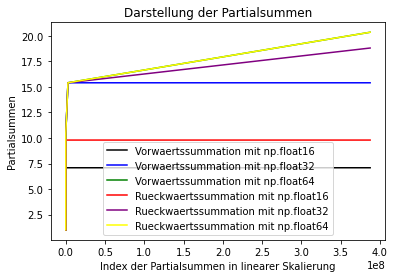
\includegraphics[width=0.6\textwidth]{plot_basis9_endwert9.png}
    \caption{Basis 9, Startwert 0, Endwert 9, Num 5}
\end{figure}

\newpage
\section{Schlussfolgerung}
Basierend auf den Ergebnissen unseres Experiments lässt sich feststellen, dass die harmonische Reihe aufgrund von Rundungsfehlern und begrenzter Genauigkeit der Fließkommazahlen auf Computern scheinbar konvergiert, obwohl sie theoretisch divergiert. Insbesondere zeigt sich, dass die Genauigkeit der Berechnung von der Wahl des Datentyps und des verwendeten Algorithmus abhängt. Während die Vorwärtssummation mit dem Datentyp \texttt{np.float32} die geringste Genauigkeit aufweist, liefert die Rückwärtssummation mit dem Datentyp \texttt{np.float64} das genaueste Ergebnis. Diese Erkenntnisse regen dazu an, weitere Optimierungen zu untersuchen, um möglicherweise eine Divergenz der harmonischen Reihe auf dem Computer nachzuweisen.

\section{Quellen}
\begin{itemize}
\item \url{https://de.wikipedia.org/wiki/Harmonische_Reihe}
\item \url{https://techwatch.de/blog/understanding-floating-point-numbers-a-comprehensive-guide-for-tech-enthusiasts/}

\end{itemize}


\end{document}
